\section{Description and Phenomenology of the Signal}
\label{sec:stop_pheno}


\subsection{Aside: SUSY Signal Grids}
\label{sec:susy_signal_grid}

\begin{figure}[!htb]
    \begin{center}
        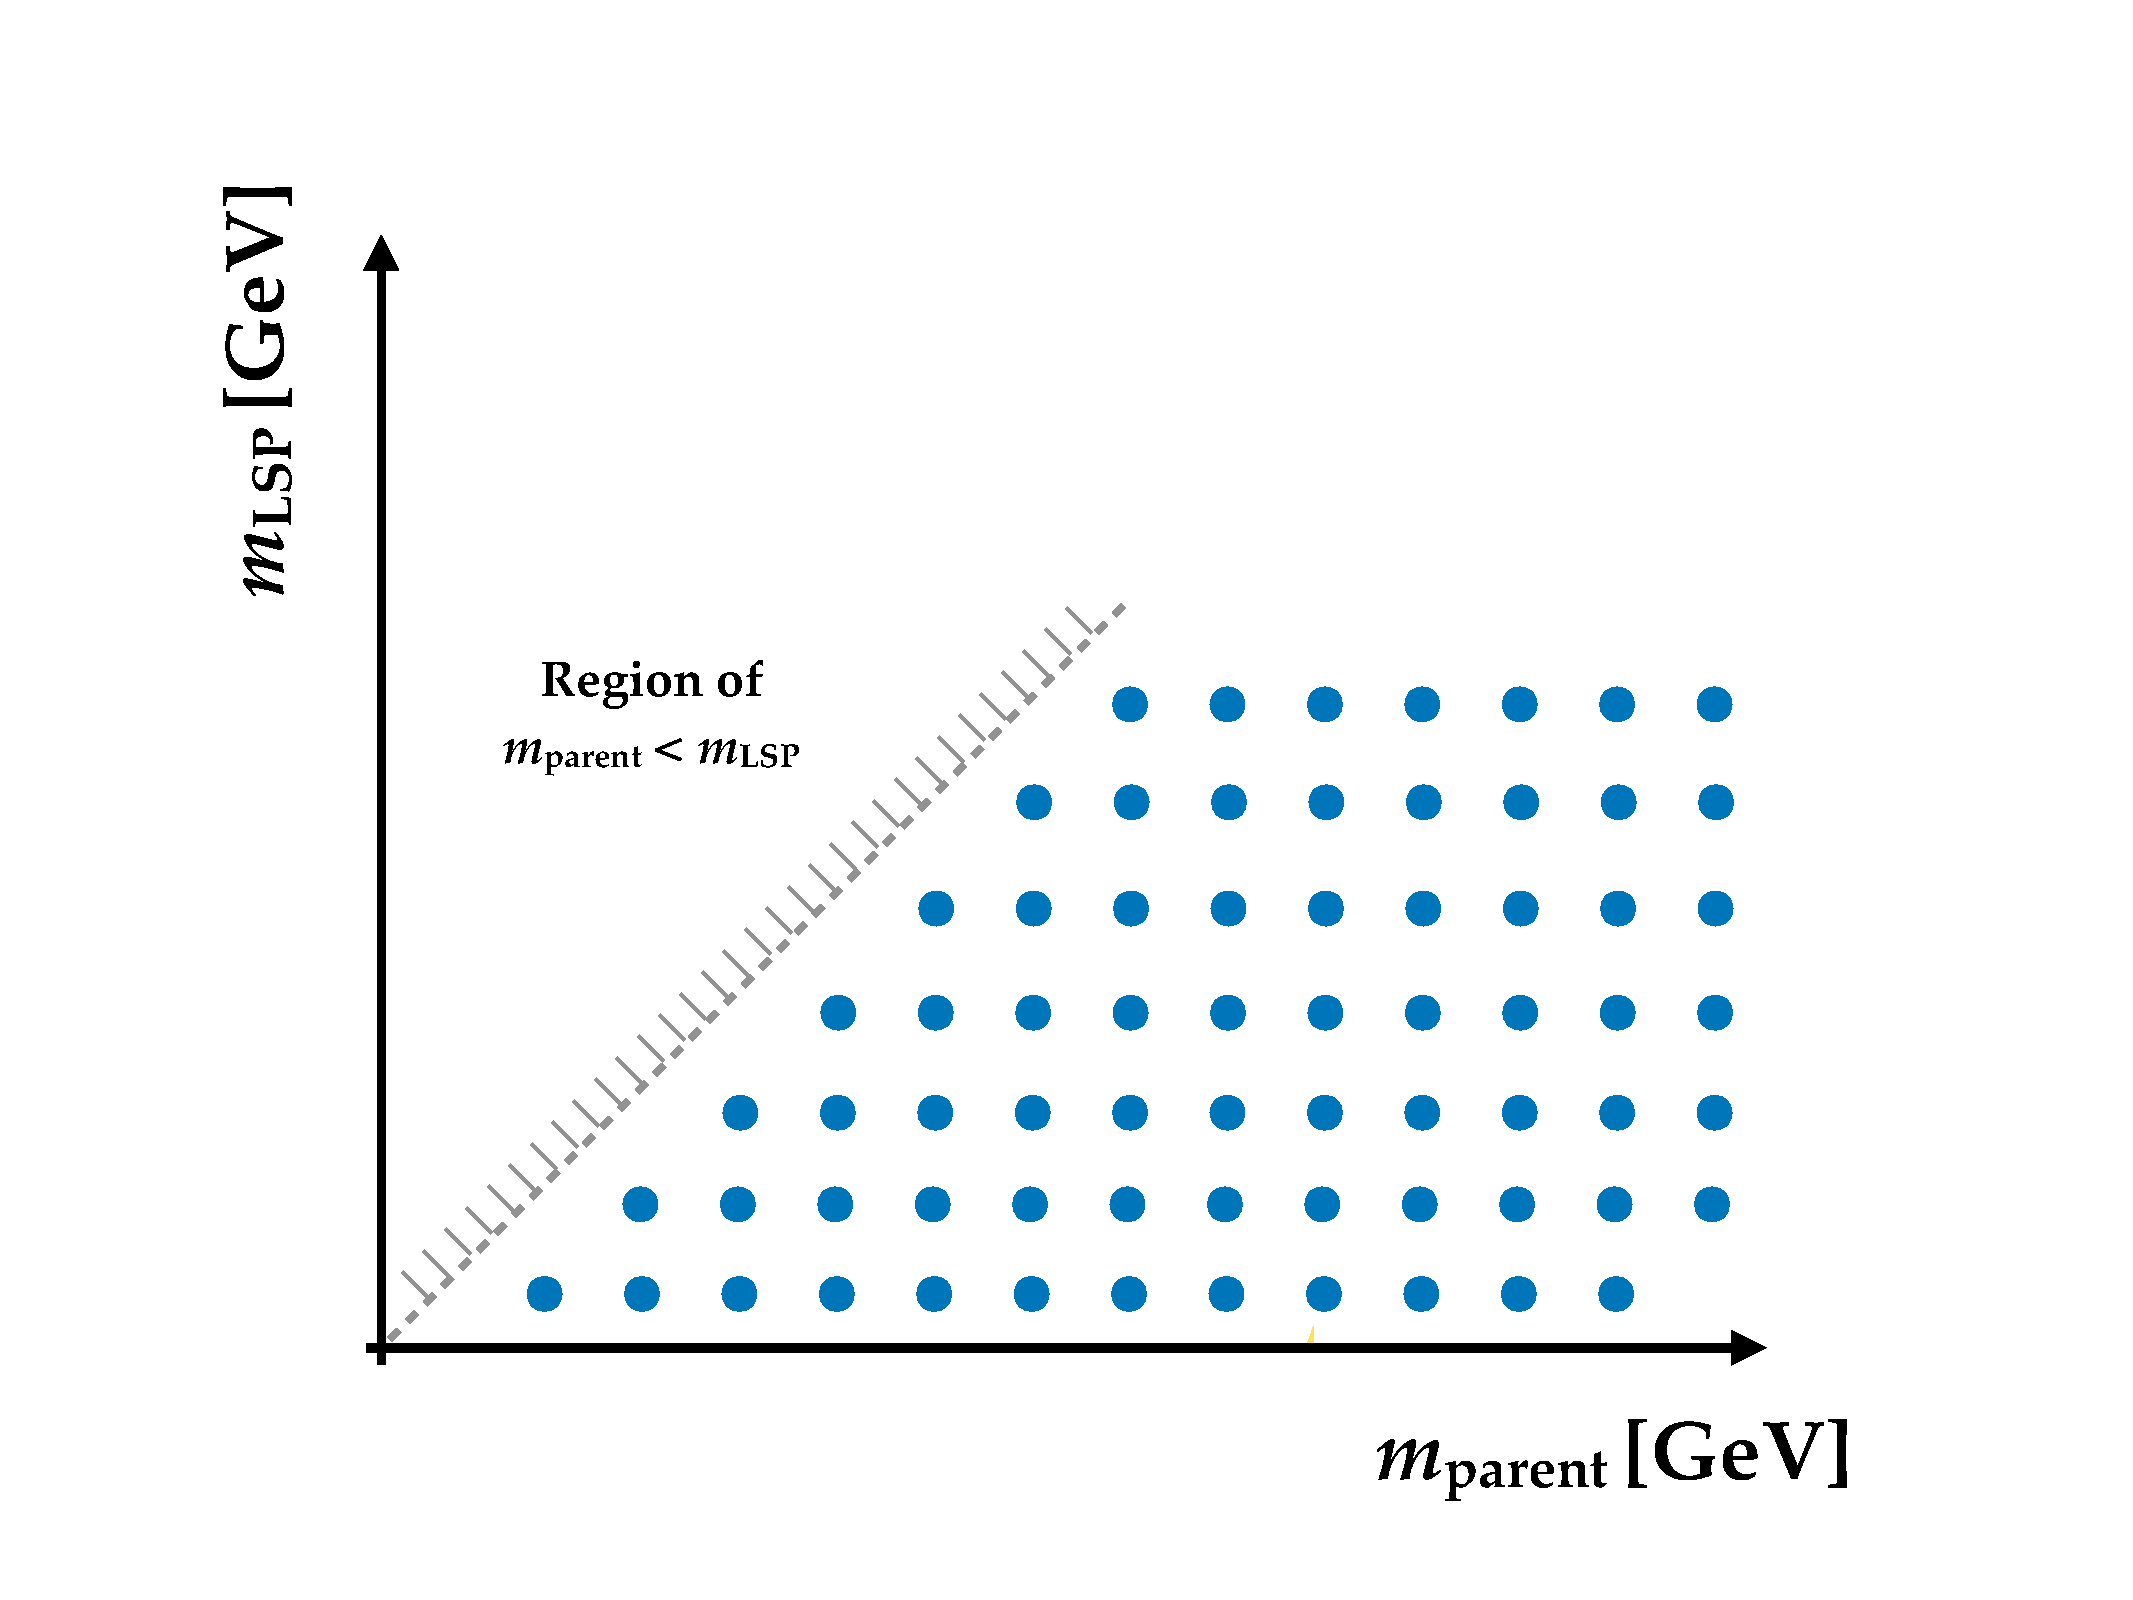
\includegraphics[width=0.6\textwidth]{figures/search_stop2l/signal/susy_signal_grid_example}
        \caption{
            Illustration of a SUSY signal grid.
            The blue points indicate points in the simplified model parameter space for which
            an individual MC-simulated sample is produced and available for use in analyses
            searching for the given type of SUSY.
        }
        \label{fig:susy_signal_grid}
    \end{center}
\end{figure}

Before the search for the \stopone can begin, MC simulated samples representing this process
must be obtained.
Once a given simplified model of the MSSM is chosen, specific points in the
$(m_{\stopone}, m_{\ninoone})$-plane are chosen and for each a separate MC simulated
sample is produced.
Each point represents a different hypothesis of SUSY, characterised by the specific masses
of the \stopone and \ninoone sparticles.
In ATLAS, this process of choosing points in the SUSY parameter space to produce MC simulated samples
is one requiring high levels of deliberation and discussion.
This is due to the fact that the simulation of complicated physics processes requires large amounts
of ATLAS' CPU resources, of which any given analysis group only has so much allocated, and so, among other things,
judicious choices about the number of events to be simulated at each point in the $(m_{\stopone}, m_{\ninoone})$-plane
must be made, as well as careful consideration of previous analyses' exclusion coverage in the same parameter space.
For this reason, the resulting SUSY `signal grids' are \textit{sparse}, as illustrated in Figure~\ref{fig:susy_signal_grid}.
Depending on how sparse the produced signal grid is, how the points are grouped, or how large each MC-sample at each
point is (in terms of number of MC events simulated), the resulting analyses' conclusions
can result in unphysical or even discontinous exclusion regions, which is clearly the case in the Run 1 searches
for the three-body decay of the \stopone, seen in Figure~\ref{fig:run1_stop_summary}.
When interpreting the results of SUSY searches, then, it is important to keep these facts in mind
so as to not over-interpret the results' statements about any fine-grained details of SUSY parameter space to
which the analyses are generally not sensitive.
Each point in a SUSY signal grid allows, rather, an analysis to make general statements about
an \textit{extended}, but still local, region of parameter space under the assumed simplified model.


%\subsection{Simulation of the Three-body Decay of the Stop Quark}
%\label{sec:stop_sim}
%
%The MC simulation of the three-body decay of the \stopone, used in the analysis discussed in 
%this chapter, is performed using \textsc{MadGraph5\_AMC@NLO}, including diagrams with up to
%two additional partons.
%In the three-body region of phase space of the \stopone decays, proceeding via off-shell
%intermediate SM top-quarks, the preservation of the \stopone left-right polarisation information
%must be handled with care.\footnote{The
%\stopone is of course a scalar particle, so it not chiral.
%The \stopL and \stopR  states that make up the \stopone and \stoptwo mass eigenstates refer, instead, 
%to their corresponding SM superpartner counterparts.
%}
%For this reason, produced \stop sparticles provided by \textsc{MadGraph5\_AMC@NLO} are decayed
%via \textsc{MadSpin}, described in Section~\ref{sec:mc_gen_afterburner}, which properly
%propagates the polarisation information of the massive \stopone particle into the
%off-shell and intermediate SM top-quark to which it decays, such that the kinematics of the
%$W$-boson ($\ell \nu$ system) and $b$-quark are correct.
%\textsc{Pythia} is used for the showering and fragmentation.

\subsection{Description of the Three-body Decay Final State}
\label{sec:stop_final_state}

\begin{figure}[!htb]
    \begin{center}
        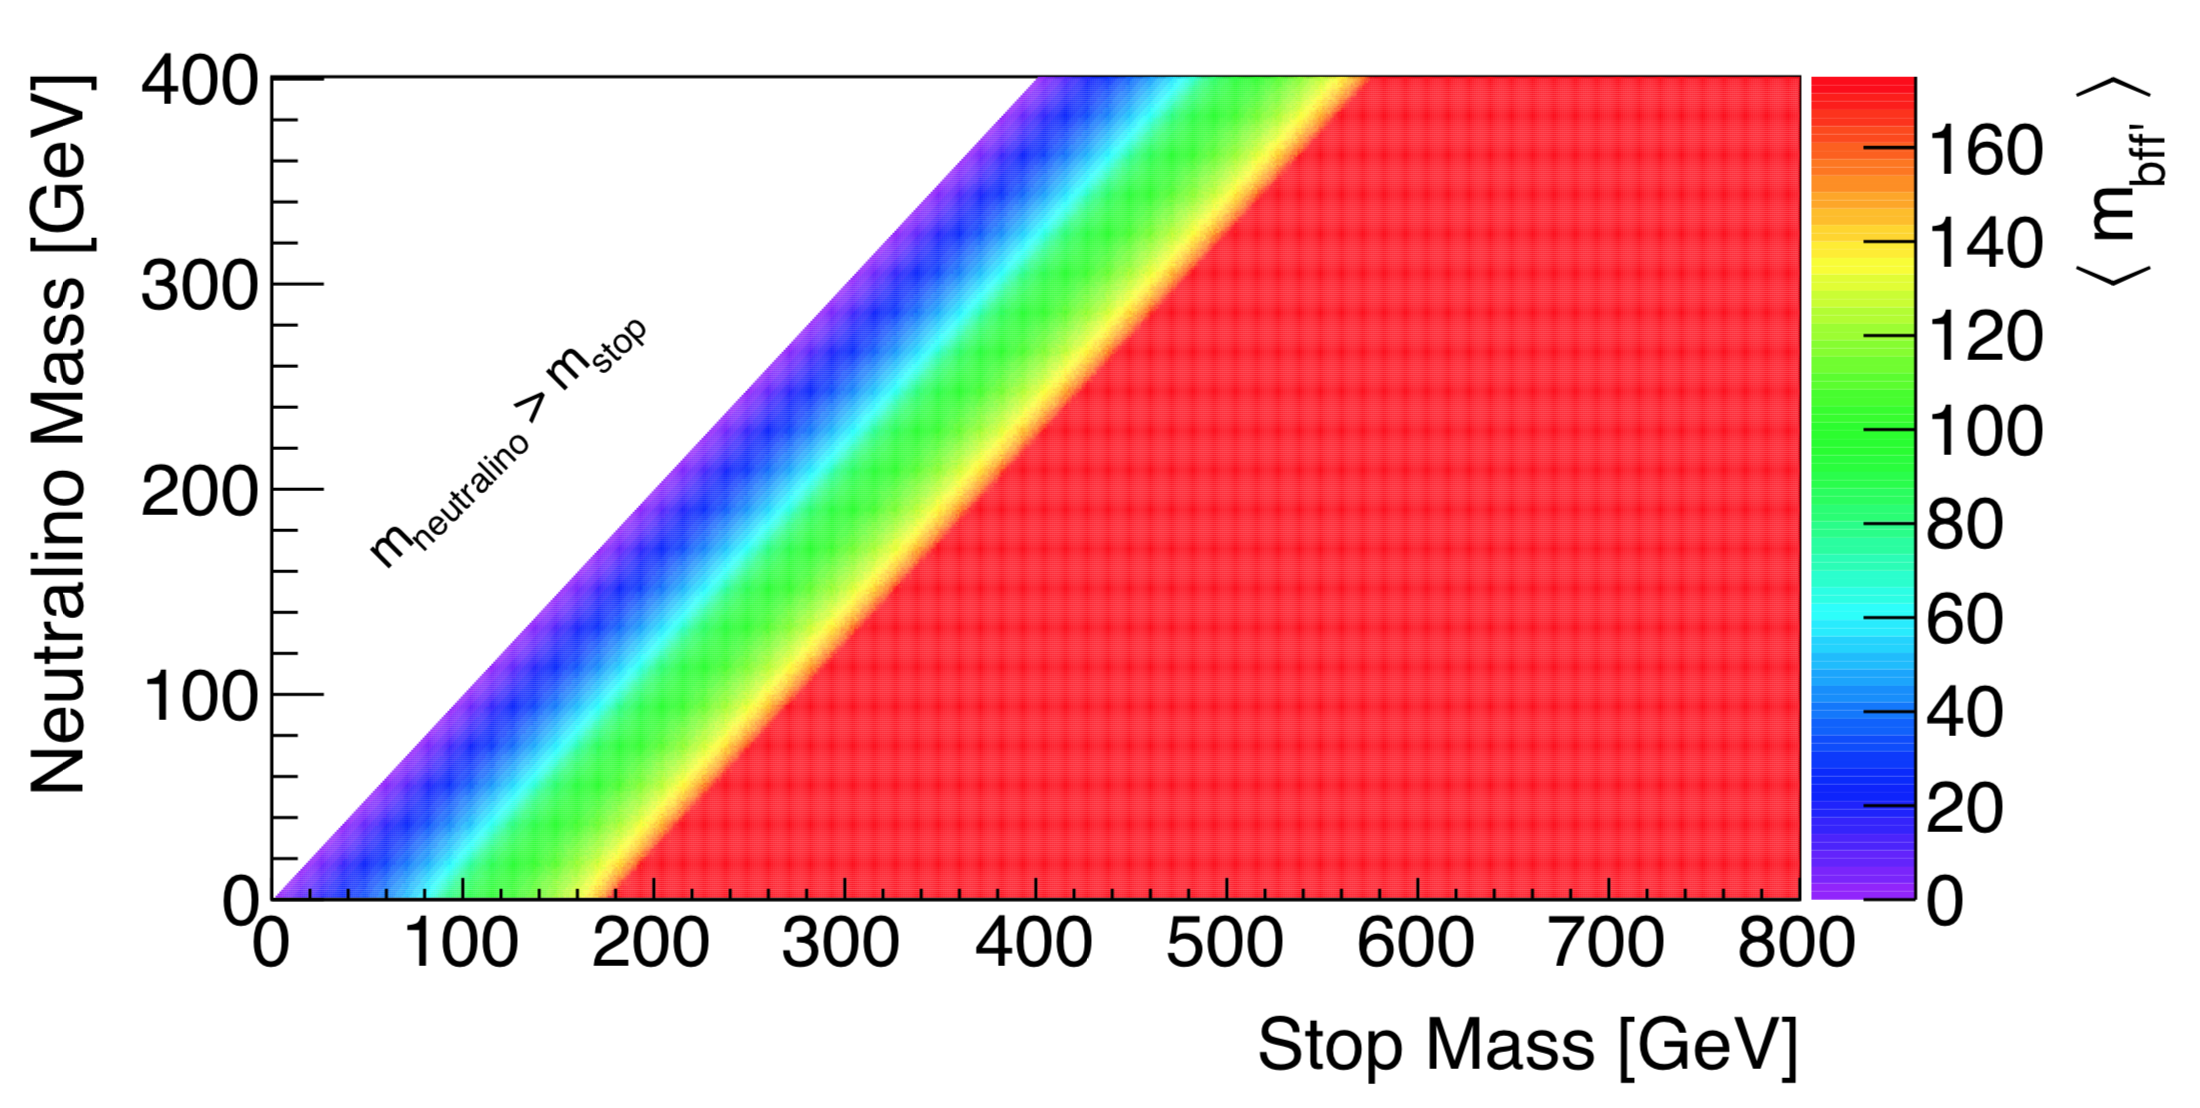
\includegraphics[width=0.75\textwidth]{figures/search_stop2l/nachman_stop_phase_space}
        \caption{
            Average invariant mass of the $b$-quark and SM fermions ($f f^{\prime}$) in the
            final state of the $\stopone \rightarrow b f f^{\prime} \ninoone$ decay, as a function of the mass
            of the \stopone and \ninoone particles.
            Figure taken from Ref.~\cite{Nachman:2016qyc}.
        }
        \label{fig:stop_phase_space}
    \end{center}
\end{figure}

In the three-body decays, the \stopone is assumed to decay via an off-shell SM top quark.
This is a kinematically suppressed region of phase space, as illustrated in Figure~\ref{fig:stop_phase_space},
which shows the average invariant mass of the \stopone decay products across the
two-, three-, and four-body decay regions of the $(m_{\stopone}, m_{\ninoone})$-plane (c.f. Figure~\ref{fig:stop_boundaries}).
In Figure~\ref{fig:stop_phase_space} the onset of the restricted phase space is clearly
visible as one drops beneath the $\sdiff = m_{\text{top}}$ line, at which point the final
state particle kinematics change rapidly.

The restricted phase space of the three-body \stopone decays has a large
impact on the analyses searching for the \stopone.
The $b$-quark children of the \stopone decays have decreasing momenta as one
moves from the $\sdiff = m_{\text{top}}$ kinematic boundary to that of $\sdiff = m_{W}$.
As a result, the $b$-jets that arise as a result of the $b$-quark hadronization process
are difficult to identify efficiently given the minimum 20\,\GeV~\pT~thresholds typical
of the ATLAS jet reconstruction and flavor-tagging identification algorithms.
This is illustrated in Figure~\ref{fig:stop_nbjets}, showing the $b$-tagged jet multiplicities
for various \stopone decay scenarios and how they compare to the dominant SM backgrounds.
As $\sdiff \rightarrow m_W$, the flavor-tagging algorithms are unable to identify the $b$-jets,
and the final state is kinematically similar to that of SM $WW$ production.

\begin{figure}[!htb]
    \begin{center}
        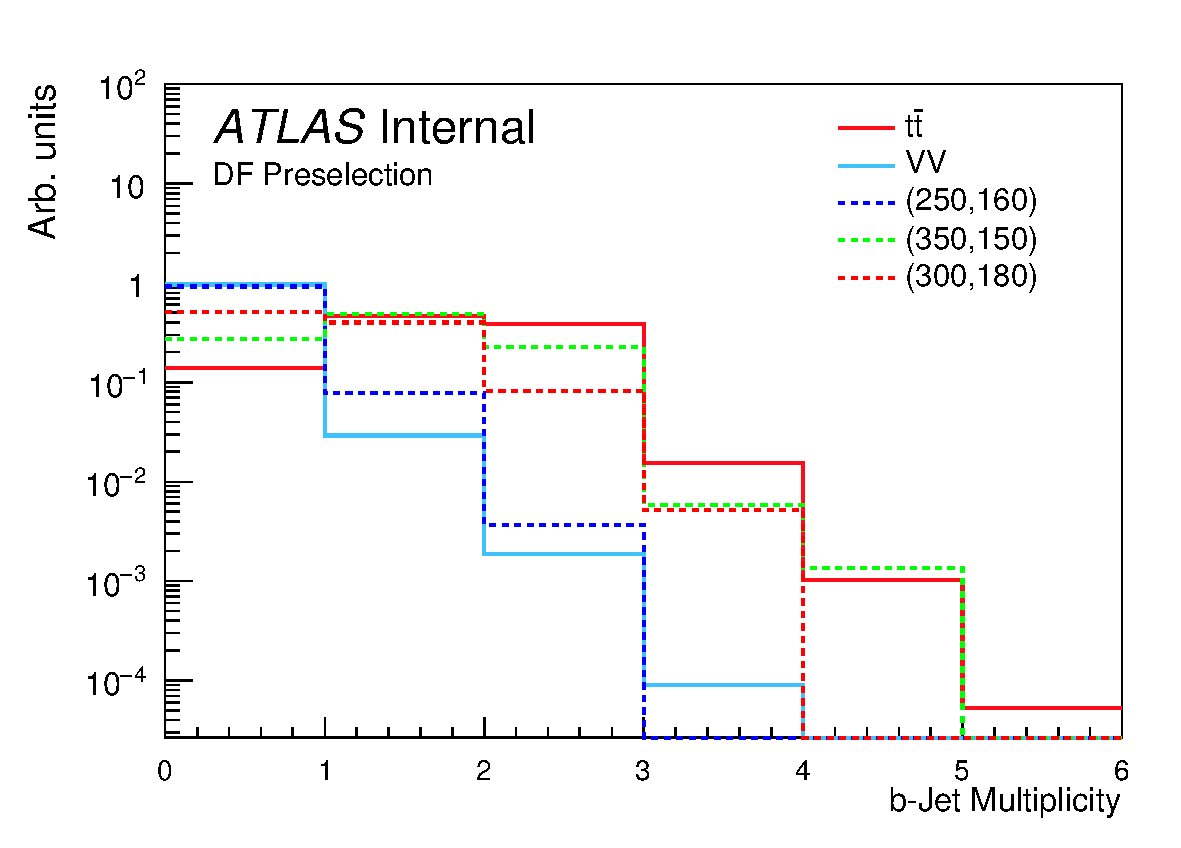
\includegraphics[width=0.7\textwidth]{figures/search_stop2l/strategy/comp_plots/dfpresel_nBJets}
        \caption{
            Normalised $b$-tagged jet multiplicity distributions for three \stopone signals (dashed lines),
            indicated by their position in the $(m_{\stopone}, m_{\ninoone})$-plane in the legend,
            and SM \ttbar~(solid red red) and diboson (VV) (solid blue line) production.
            It can be seen that the \stopone decays with $\sdiff \sim m_{\text{top}}$ have $b$-tagged jet
            multiplicities similar to that of SM \ttbar production.
            The \stopone decays with $\sdiff \rightarrow m_W$ tend to have zero reconstructed $b$-tagged jets.
            The selection, `DF Preselection', in the plot is that described in Table~\ref{tab:stop_preselection}.
        }
        \label{fig:stop_nbjets}
    \end{center}
\end{figure}

The \ninoone children of the \stopone decays, as with the $b$-quarks, also exhibit diminishing
momenta as one traverses the three-body region from the $\sdiff = m_{\text{top}}$ kinematic boundary to that of $\sdiff = m_W$.
As a result, the three-body \stopone decays do not have the typical signature of large
amounts of missing transverse momentum, typical of $R$-parity conserving SUSY decays.
The reduced impact of the \ninoone particles on the magnitude of the missing transverse momentum
furthers the three-body \stopone decays' resemblance to those of SM $WW$ production, in that
the primary carriers of missing transverse momentum are the neutrinos from the leptonic decays
of the $W$ bosons.

The three-body region allows for the on-shell production of the $W$ bosons.
For this reason, the leptons and neutrinos from their decay are not kinematically suppressed
in the same way as the $b$-quarks and \ninoone.
Their kinematics are therefore typical, in scale, to those of SM \ttbar~and $WW$ production.
